%%%%%%%%%%%%%%%%%%%%%%%%%
% Dokumentinformationen %
%%%%%%%%%%%%%%%%%%%%%%%%%


\newcommand{\trtitle}{App f\"ur Dienstabmachungen}
\newcommand{\scrartclScrreprt}{scrartcl}
%!TEX TS-program = pdflatex
\documentclass[fontsize=12pt]{\scrartclScrreprt}
\usepackage[utf8]{inputenc}

\usepackage[numbers]{natbib}
\usepackage{lmodern}
\usepackage[T1]{fontenc}
\usepackage[ngerman, num, orig]{isodate}
\usepackage[ngerman]{babel}   
\monthyearsepgerman{\,}{\,} 



% eigene commands

\newcommand{\texttodo}[1]{\textcolor{red}{Todo: #1}}


% Kompaktes Itemize
\usepackage{enumitem}
\newlist{compactitemize}{itemize}{1}
\setlist[compactitemize]{label=\textbullet, nosep, leftmargin=10pt}

\usepackage{layout}
\setlength{\parindent}{0em}

\usepackage{amssymb,amsmath,fancybox,graphicx,wrapfig,color,lastpage,fancyhdr,verbatim,epstopdf,a4wide}

\usepackage{tabularx}
\usepackage{setspace}
\usepackage{epsfig}
\usepackage{pst-pdf}
\usepackage{pst-all}
\usepackage{supertabular}{\tiny }
\usepackage[font=small,labelfont=bf]{caption}
\usepackage{subcaption}
\usepackage{footnote}
\usepackage{float}
\usepackage{multirow}
\usepackage{etex}
\usepackage{pdfpages}
\usepackage{color} 
\usepackage{placeins} 
\usepackage{booktabs}
\usepackage{pdflscape}

\usepackage[hyphens]{url}	%URL handling und darstellung
\urlstyle{tt}

\usepackage[pdftitle={\trtitle},
						pdfauthor={Philipp Riedel},
						pdfcreator={TexMate, LaTeX with hyperref},
						pdfsubject={\trtitle},
						plainpages=false,
						pdfpagelabels,
						colorlinks,
						linkcolor=black,
						filecolor=black,
						citecolor=black,
						urlcolor=blue]{hyperref}

\usepackage[makeroom]{cancel}
\usepackage{array}
\usepackage{trfsigns}
\usepackage{textcomp}

\title{\trtitle}
\subtitle{(Planung)}
\author{(Philipp Riedel \& co)}

% Möglichst keine Ergänzungen hier, sondern in header.tex
\begin{document} 
 

% Römische Nummerierung für Sonderseiten, wie Verzeichnisse und Anhang
\pagenumbering{Roman}

% Titelblatt

\maketitle


% Inhaltsverzeichnis
\tableofcontents
\thispagestyle{empty}
% Nummerierung von roemisch auf arabisch umschalten und roemische
% zwischenspeichern
\newpage
\pagenumbering{arabic}


\section{Einleitung}

Diese Dokumentation soll während des ganzen Projekt ergänzt und nachgeführt werden.
\subsection{Zweck dieser Applikation}
\begin{itemize}
\item Diese App ist für Verkündiger gedacht.
\item Es soll nicht als Ersatz der Dienstabmachungen mit der eigenen Versammlung dienen.
\item Diese App soll lediglich das finden eines Dienstpartners vereinfachen, wenn Verkündiger eine kurzfristige Dienstabsage erhalten oder wenn niemand für den Dienst zu einer bestimmten Zeit gefunden werden konnte.
\item Die App hat ihr Anwendungsgebiet innerhalb einer bestimmten Region, welche im Moment auf den Raum Zürich beschränkt ist.
\item Diese App soll auch Abmachungen mit einer Sprache, die nicht der Muttersprache entspricht, ermöglichen.
\item Der Grundgedanke die Dienstgruppe und die Einheit zu fördern soll bei der Implementierung der Applikation berücksichtigt werden.
\end{itemize}

\subsection{Projektaufbau}

Dieser Aufbau ist noch abhängig von gewissen Grundsatzentscheiden, ausserdem ist er eventuell noch nicht Vollständig \texttodo{überarbeiten, nach vorgehens entscheid (cross plattform, je ein app, gwt usw.)}

\begin{center}
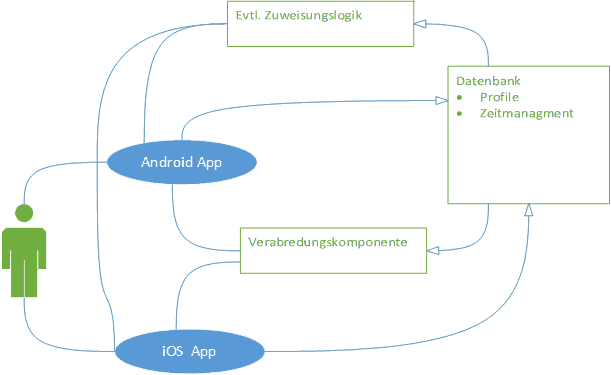
\includegraphics[width=0.75\textwidth]{bilder/useCase.png}
\end{center}

\section{Vorabklärungen}

\subsection{Zusammenfassung}
\begin{tabularx}{\textwidth}{lX}
Task  & Stand \\\hline
Bedürfnis & das Bedürfnis ist vorhanden \\
Teilnahme Abschätzung für Gelingen & Teilnehmerzahl $n \geqslant 100$, Pioniere $n_p \geqslant 50$\\
Aufwand & \texttodo{ToDo Cristian oder Anna-Nina} \\
Installation auf Android - und iOS Systeme & Android stellt kein Problem dar, bei AppStore fallen zusätzliche Kosten an, ausserdem ist man der Willkür von Apple ausgesetzt. Da aber viele ein iPhone besitzen muss auch für iOS eine App zur Verfügung gestellt werden.\\
Datenbank &\texttodo{Anna-Nina bitte eine Struktur vorschlagen, Aufwand, Unterhalt, Kosten und Risiken}\\
Sicherheit &  \texttodo{Philipp und Sam besprechung des Aufbaus der App mit einbezug von Theokratischen Argumenten}\\
\end{tabularx}

\subsection{Bedürfnis}

\paragraph{Wie gross ist das Bedürfnis nach dieser Applikation} bei vielen Verkündigern kommen Absagen relativ häufig vor, bei Pionieren 1 bis 2 mal pro Woche. Auch das finden von Abmachungen unter der Woche kann eine Herausforderung sein.

\subsection{Teilnahme Abschätzung für Gelingen}
\paragraph{Wie viele absagen braucht es pro Woche damit die Applikation einen Nutzen hat} Es gibt pro Tag in etwa die drei Hauptterminzeiten Morgen, Nachmittag und Abend. Samstag Abend wird weggelassen und sonntags zählt nur als eine Terminzeit. Somit ergeben sich 18 Termine pro Woche. Damit es öfters vorkommt das bei den Hauptterminzeiten eine Übereinstimmung mit $\pm\varepsilon$ gegeben ist, sollte mit 60 bis 100 Absagen oder nicht Finden einer Abmachung pro Woche gerechnet werden. Dies sollte mit einer Teilnehmerzahl $n \geqslant 100$ und davon $n_p \geqslant 50$ Pionieren erreicht werden.

\subsection{Aufwand}
\paragraph{Aufwand für Programmierung und Unterhalt} Der Aufwand muss im Verhältnis zum Nutzen stehen. \texttodo{Cristian oder Anna-Nina: bitte hier eine Zeitabschätzung getrennt nach Erstellen der Applikation sowie deren Unterhalt erstellen}

\subsection{Installation der App}
\paragraph{Bedignungen für die Installation auf Android - und iOS Systeme}
\begin{itemize}
\item Bei einem Android System ist es kein problem die Applikation auf ein File-Server zum Download anzubieten. Der Nutzer muss nur bei der Installation zustimmen, dass er die unbekannte App als vertrauenswürdig hält.
\item Bei einem iOS Stystem muss über den AppStore gegangen werden.  Zum Veröffentlichen der App im App Store ist eine kostenpflichtige Registrierung beim iOS Developer Program notwendig. Apple unterzieht jede eingesandte App einer Überprüfung und erteilt anschließend in der Regel die Freigabe für den App Store. Dies ist die einzige Möglichkeit die App zu verbreiten wenn die Apple Geräte keinem Jailbreak unterzogen wurden \cite{appStore}. Für das Anbieten von Apps im AppStore fallen kosten von 99.-\$ an.
\end{itemize}
Trotz Mehraufwand und zusätzlichen Kosten muss wegen der hohen Anzhal von iPhone besitzer auch für iOS eine App zur Verfügung gestellt werden.

\subsection{Datenbank}
\paragraph{Nutzen und Aufwand einer Datenbank}Da Profile erstellt werden müssen damit eine effiziente Zuordnung gemacht werden kann muss eine Datenbank Struktur vorhanden sein.

\texttodo{Anna-Nina bitte eine Struktur vorschlagen, Aufwand, Unterhalt, Kosten und Risiken}

\subsection{Sicherheit}
\paragraph{Abklärungen zur Sicherheit in Abhängikeit der Daten} Die Sicherheitsanforderungen hängen primär auch von den gespeicherten Daten ab. Die gespeicherten Attribute eines Verkündigers müssen noch Evaluiert werden, dies wird von Samuel Vontobel und Philipp Riedel mit eventueller Einbeziehung von weiteren Brüdern durchgeführt. Die Attribute sind wiederum abhängig von der Auslegung der Applikation. Telefonnummern werden zum Beispiel nicht benötigt wenn eine Appinterner Kommunikationsablauf zur Verabredung bereitgestellt wird. Namen würden z.B. nicht benötigt wenn eine Anonyme Zuweisung erfolgt. Eine Versammlungszugehörigkeit wird nur dann benötigt wenn bei einer automatischen Zuteilung die eigene Versammlung als Zulteilungspriorität gilt usw. 

\texttodo{Philipp und Sam besprechung des Aufbaus der App mit einbezug von Theokratischen Argumenten}\newline

\texttodo{Danach: Anna-Nina: Sicherheitsvorschlag, verschlüsselung? profile mit Password versehen? usw.}
\section{Anforderungen}

\begin{itemize}
\item Standorthandling
\begin{itemize}
\item Wenn es möglich ist bei iOS und/oder Android ein generelles blockieren der Preisgabe des Standortes einzustellen muss der User die Möglichkeit bekommen manuelle seinen Standort einzugeben
\end{itemize}
\item Toleranzhandling, die verfügbaren Zeiten müssen nicht exakt übereinstimmen, die Toleranz $\varepsilon$ sollte von der Verabredungsdauer abhängig sein.
\item \texttodo{evtl. Zuteillogik}
\item Auch bei Taskabschuss mit einem Taskmanagertool muss die Applikation ansprechbar bleiben, damit eine neu eingetroffene Zeitübereinstimmung ein Pop-up generieren kann.
\item \texttodo{evtl. weitere} 
\end{itemize}




\subsection{Fragen zu weiteren Anforderungen und Bestimmungen}

\subsubsection{Technische}


\begin{itemize}
\item Ablehnen wie handeln
\item eine Verabredungskommunikation die den Dialog standardisiert und vereinfacht bereitstellen
\item Handling von keine Reaktion
\item Handling von $n_v>2$ bei geraden und ungeraden $n_v$
\item Verabredungsabwicklung
\item Statistik mitführen
\item Zeitwahl auf x min begrenzen
\item Wählbar ob Verabredungskommunikation oder Telefonnummer Bekanntgabe
\end{itemize}

\paragraph{Ablehnen wie handeln}
\vspace{3cm} 

\paragraph{eine Verabredungskommunikation die den Dialog standardisiert und vereinfacht bereitstellen}
\vspace{3cm} 

\paragraph{Handling von keine Reaktion}
\vspace{3cm} 

\paragraph{Handling von $n_v>2$ bei geraden und ungeraden $n_v$}
\vspace{3cm} 

\paragraph{Verabredungsabwicklung}
\vspace{3cm} 

\paragraph{Statistik mitführen}
\vspace{3cm} 

\paragraph{Zeitwahl auf x min begrenzen}
\vspace{3cm} 

\paragraph{Wählbar ob Verabredungskommunikation oder Telefonnummer Bekanntgabe}
\vspace{3cm} 

\subsubsection{Theokratische}


\begin{itemize}
\item Wie wird sichergestellt das nicht langfristige Verabredungen ausschliesslich über die Applikation getätigt werden, damit nicht Ungerechtigkeiten gegenüber solchen, die nicht mit machen können oder wollen, entstehen
\item Handhabung der Verteilung der App, Gefahr das sich ausgeschlossene einschleichen und ähnliches
\item Sichtbarkeit der Namen, Gefahr das spezielle Charakteren öfters abgelehnt werden, diese dies auf irgend eine Art und Weise herausfinden und sich gemobbt fühlen
\item eine Suchfunktion integrieren, damit solche zur Verfügung stehen könnten, sich solchen die niemanden finden anbieten können
\end{itemize}

\paragraph{Wie wird sichergestellt das nicht langfristige Verabredungen ausschliesslich über die Applikation getätigt werden, damit nicht Ungerechtigkeiten gegenüber solchen die nicht mit machen können oder wollen entstehen}
\vspace{3cm} 

\paragraph{Handhabung der Verteilung der App, gefahr das sich ausgeschlossene einschleichen und ähnliches}
\vspace{3cm} 

\paragraph{Sichtbarkeit der Namen, Gefahr das spezielle Charakteren öfters abgelehnt werden, diese dies auf irgend eine Art und Weise herausfinden und sich gemobbt fühlen}
\vspace{3cm} 

\paragraph{eine Suchfunktion integrieren, damit solche zur Verfügung stehen könnten, sich solchen die niemanden finden anbieten können}
\vspace{3cm} 


% Nummerierung wieder auf roemisch umschalten
%\newpage
%\pagenumbering{Roman}
%\setcounter{page}{\value{roemisch}}



\end{document}
